\documentclass[aspectratio=169]{beamer}

\usetheme{Madrid}
\usecolortheme{seahorse}
\usepackage{listings}
\usepackage{tikz}
\usetikzlibrary{arrows.meta, shapes.geometric, positioning, fit, backgrounds}
\usepackage{booktabs}
\usepackage{xcolor}
\usepackage{graphicx}

% color palette
\definecolor{zblue}{RGB}{31, 78, 121}
\definecolor{zaccent}{RGB}{0, 112, 192}
\definecolor{zwarn}{RGB}{192, 80, 77}
\definecolor{zok}{RGB}{70, 130, 80}
\definecolor{zgray}{RGB}{89, 89, 89}
\definecolor{codebg}{RGB}{245, 246, 250}

\setbeamercolor{frametitle}{bg=zblue, fg=white}
\setbeamercolor{title}{bg=zblue, fg=white}
\setbeamercolor{structure}{fg=zaccent}
\setbeamercolor{block title}{bg=zblue!80, fg=white}
\setbeamercolor{block body}{bg=zblue!8}
\setbeamercolor{alerted text}{fg=zwarn}

\lstdefinestyle{cpp}{
  language=C++,
  basicstyle=\ttfamily\scriptsize,
  keywordstyle=\bfseries\color{zblue},
  commentstyle=\itshape\color{zgray},
  stringstyle=\color{zok!80!black},
  backgroundcolor=\color{codebg},
  frame=single, framerule=0.4pt, rulecolor=\color{zaccent!40},
  xleftmargin=4pt, xrightmargin=4pt,
  breaklines=true, breakatwhitespace=false,
  tabsize=3, showstringspaces=false,
  morekeywords={auto,const,std,vector,stringstream,uint64_t,NGuiKey,EPointName,GuiPackSubjectBasic_t}
}
\lstdefinestyle{python}{
  language=Python,
  basicstyle=\ttfamily\scriptsize,
  keywordstyle=\bfseries\color{zblue},
  commentstyle=\itshape\color{zgray},
  stringstyle=\color{zok!80!black},
  backgroundcolor=\color{codebg},
  frame=single, framerule=0.4pt, rulecolor=\color{zaccent!40},
  xleftmargin=4pt, xrightmargin=4pt,
  breaklines=true, showstringspaces=false, tabsize=4
}
\lstdefinestyle{json}{
  basicstyle=\ttfamily\scriptsize,
  keywordstyle=\color{zblue},
  stringstyle=\color{zok!80!black},
  backgroundcolor=\color{codebg},
  frame=single, framerule=0.4pt, rulecolor=\color{zaccent!40},
  xleftmargin=4pt, xrightmargin=4pt,
  breaklines=true, showstringspaces=false
}

\title{ZandrEA Named Write Path}
\subtitle{\texttt{/profiles} and conversion to backend point order}
\author{}
\date{\today}

\begin{document}

\begin{frame}
  \titlepage
\end{frame}

\begin{frame}{Roadmap}
  \tableofcontents
\end{frame}

% -----------------------------------------------------------------------------
\section{What Changed}

\begin{frame}{The Write Contract Problem}
\begin{columns}[T]
\column{0.48\textwidth}
\begin{block}{Old contract}
  Clients posted numeric arrays to \texttt{/ctrl/sampletimestep}.
  The order had to match libEA's internal point registration order.
\end{block}

\vspace{0.5em}
\begin{block}{Failure mode}
  If a client put the right values in the wrong order, the backend accepted
  the array and wrote values to the wrong \texttt{ADataChannel}s.
\end{block}

\column{0.48\textwidth}
\begin{block}{New contract}
  Clients fetch \texttt{/profiles}, then post named values to
  \texttt{/ctrl/sampletimestep-named}.
\end{block}

\vspace{0.5em}
\begin{block}{Compatibility boundary}
  The backend still receives the same ordered vector through
  \texttt{SetCoincidentInputsForSubject}. The REST handler now performs the
  name-to-order conversion.
\end{block}
\end{columns}
\end{frame}

\begin{frame}{High-Level Flow}
\begin{center}
\resizebox{0.94\linewidth}{!}{%
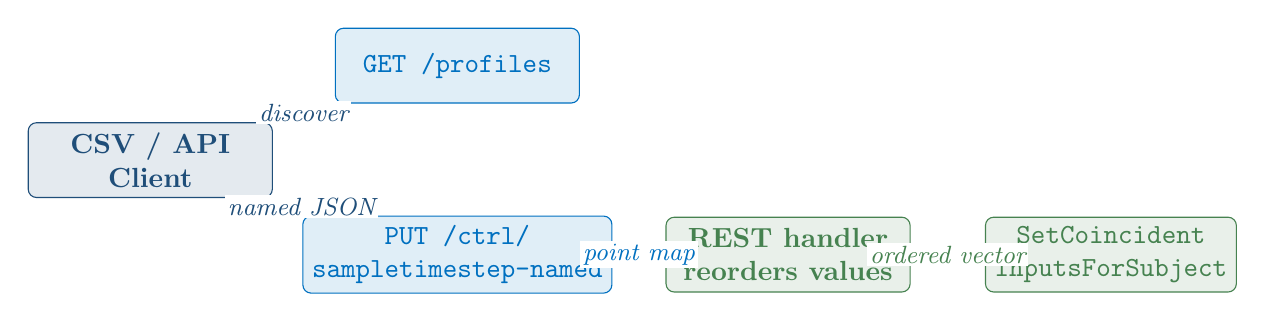
\begin{tikzpicture}[
  box/.style={rectangle, rounded corners=3pt, draw=#1, fill=#1!12,
              minimum width=3.1cm, minimum height=0.95cm, align=center,
              font=\normalsize\bfseries, text=#1},
  arr/.style={-{Stealth[length=7pt]}, very thick, #1},
  lbl/.style={font=\small\itshape, midway, fill=white, inner sep=1pt}
]
\node[box=zblue]   (client) at (0,0) {CSV / API\\Client};
\node[box=zaccent] (prof)   at (3.9,1.2) {\texttt{GET /profiles}};
\node[box=zaccent] (named)  at (3.9,-1.2) {\texttt{PUT /ctrl/}\\ \texttt{sampletimestep-named}};
\node[box=zok]     (order)  at (8.1,-1.2) {REST handler\\reorders values};
\node[box=zok]     (port)   at (12.2,-1.2) {\texttt{SetCoincident}\\ \texttt{InputsForSubject}};

\draw[arr=zblue] (client) -- node[lbl]{discover} (prof);
\draw[arr=zblue] (client) -- node[lbl]{named JSON} (named);
\draw[arr=zaccent] (named) -- node[lbl]{point map} (order);
\draw[arr=zok] (order) -- node[lbl]{ordered vector} (port);
\end{tikzpicture}
}
\end{center}
\end{frame}

% -----------------------------------------------------------------------------
\section{\texttt{/profiles}}

\begin{frame}[fragile]{\texttt{/profiles}: Profile Entries}
\begin{columns}[T]
\column{0.55\textwidth}
\begin{lstlisting}[style=json]
{
  "profiles": {
    "AHU_ibal": {
      "label_id": "AHU_ibal",
      "label": "AHU",
      "points": [
        "Pressure_static_air_supply",
        "Temperature_air_outside",
        "Position_damper_mixingBox",
        "Temperature_air_mixed"
      ]
    }
  }
}
\end{lstlisting}

\column{0.41\textwidth}
\vspace{0.5em}
\begin{block}{What a profile means}
  \texttt{profiles} is keyed by stable profile id. Each value is a
  de-duplicated write contract: model label plus the ordered list of point
  names the backend expects.
\end{block}

\vspace{0.5em}
\small The point strings are the same \texttt{EPointName} strings accepted by
the named write endpoint.
\end{columns}
\end{frame}

\begin{frame}[fragile]{\texttt{/profiles}: Subject Entries}
\begin{columns}[T]
\column{0.54\textwidth}
\begin{lstlisting}[style=json]
{
  "subjects": [
    {
      "key": 618,
      "name": "VAV-1",
      "idtext": "VAV-1",
      "profile": "VAV_ibal",
      "label_id": "VAV_ibal",
      "label": "VAV",
      "points": [
        "Pressure_static_air_supply",
        "Temperature_air_supply",
        "Temperature_air_discharge",
        "Temperature_air_zone"
      ]
    }
  ]
}
\end{lstlisting}

\column{0.42\textwidth}
\vspace{0.4em}
\begin{block}{Why subjects repeat points}
  The profile list is cacheable by model contract. The subject list maps concrete
  runtime \texttt{NGuiKey}s to that profile and repeats the point order for a
  direct upload path.
\end{block}
\end{columns}
\end{frame}

\begin{frame}[fragile]{Building \texttt{/profiles} in \texttt{handler.cpp}}
\begin{columns}[T]
\column{0.58\textwidth}
\begin{lstlisting}[style=cpp]
for (auto const& skey : domain.subjectKeys) {
  GuiPackSubjectBasic_t subject =
    p_Port->SayInfoFromSubject(skey);

  auto points =
    p_Port->SayInputPointNameOrderExpectedBySubject(skey);

  auto label_id = subject.ownLabelId;
  auto label = subject.infoText_byCR.empty()
    ? std::string("")
    : subject.infoText_byCR[0];

  // reuse profile when label_id and points match
  // otherwise create a deterministic profile id
}
\end{lstlisting}

\column{0.38\textwidth}
\vspace{0.4em}
\begin{block}{Important source of truth}
  \texttt{SayInputPointNameOrderExpectedBySubject} asks libEA for the actual
  registered input order. The API does not invent a new order.
\end{block}
\end{columns}
\end{frame}

% -----------------------------------------------------------------------------
\section{Client Message}

\begin{frame}[fragile]{Client Adapter: CSV Header to Named Values}
\begin{columns}[T]
\column{0.53\textwidth}
\begin{lstlisting}[style=python]
CSV_COLUMN_MAP = {
  "V1_Taz": {
    "subject": "VAV-1",
    "point": "Temperature_air_zone"
  },
  "V1_Qad": {
    "subject": "VAV-1",
    "point": "FlowRateVolume_air_vav"
  },
  "A1_Tas": {
    "subject": "AHU-1",
    "point": "Temperature_air_supply"
  }
}
\end{lstlisting}

\column{0.43\textwidth}
\vspace{0.5em}
\begin{block}{Adapter responsibility}
  Source-specific CSV names stay in the client. The server exposes canonical
  subject names, subject keys, profile ids, and point names.
\end{block}

\vspace{0.5em}
\small \texttt{build\_column\_map()} validates every mapped CSV point against
the subject's \texttt{/profiles} point list before upload.
\end{columns}
\end{frame}

\begin{frame}[fragile]{Named Upload Message}
\texttt{PUT /ctrl/sampletimestep-named}

\begin{columns}[T]
\column{0.58\textwidth}
\begin{lstlisting}[style=json]
{
  "time": 1752041880,
  "values_by_subject": [
    {
      "subject": 618,
      "values": {
        "Temperature_air_zone": 26.42,
        "Pressure_static_air_supply": 13.26,
        "FlowRateVolume_air_vav": 0.094,
        "Temperature_air_supply": 24.21,
        "Binary_zoneOccupied": 0.0
      }
    }
  ]
}
\end{lstlisting}

\column{0.38\textwidth}
\vspace{0.5em}
\begin{block}{Order no longer matters here}
  \texttt{values} is a JSON object keyed by canonical point name. It can arrive
  in any object order because the handler will read values by expected point
  name.
\end{block}
\end{columns}
\end{frame}

\begin{frame}[fragile]{Client Builds the Named Message}
\begin{columns}[T]
\column{0.60\textwidth}
\begin{lstlisting}[style=python]
def row_values_by_subject(row, column_map):
  values_by_subject_key = {}
  for column, mapping in column_map.items():
    subject = mapping["subject"]
    subject_key = subject["key"]
    values_by_subject_key.setdefault(
      subject_key, {"subject": subject, "values": {}}
    )
    values_by_subject_key[subject_key]["values"][
      mapping["point"]
    ] = float(row[column])

  return [
    {"subject": key, "values": value["values"]}
    for key, value in sorted(values_by_subject_key.items())
  ]
\end{lstlisting}

\column{0.36\textwidth}
\vspace{0.4em}
\begin{block}{Result}
  Each CSV row becomes one timestep message. Values are grouped by backend
  subject key and keyed by backend point name.
\end{block}
\end{columns}
\end{frame}

% -----------------------------------------------------------------------------
\section{Server Reordering}

\begin{frame}[fragile]{Named Handler: Validate the Envelope}
\begin{columns}[T]
\column{0.60\textwidth}
\begin{lstlisting}[style=cpp]
if (handler::get_json_value(false, jvalue,
      querystringmap, U("values_by_subject"),
      valuesbysubject) &&
    handler::get_json_value(false, jvalue,
      querystringmap, U("time"), reply, timestamp)) {

  std::tm tm;
  localtime_s(&tm, &timestamp);
  p_Port->SetTimeStampInDomain(tm);

  for (const auto& json_o : valuesbysubject.as_array()) {
    subjectkey =
      json_o.at(U("subject")).as_number().to_uint64();
    NGuiKey subject(subjectkey);
    ...
  }
}
\end{lstlisting}

\column{0.36\textwidth}
\vspace{0.4em}
\begin{block}{Same transaction shape}
  Set the domain timestamp, load all coincident inputs, then call
  \texttt{SingleStepDomainOnTimeAndInputs()} once.
\end{block}
\end{columns}
\end{frame}

\begin{frame}[fragile]{The Reordering Step}
\texttt{EAd/handler.cpp}: \texttt{/ctrl/sampletimestep-named}

\begin{columns}[T]
\column{0.62\textwidth}
\begin{lstlisting}[style=cpp]
points =
  p_Port->SayInputPointNameOrderExpectedBySubject(subject);

auto value_object = values.as_object();
std::vector<double> dlist;

for (auto const& point : points) {
  auto point_key = json_pointname(point).as_string();
  auto value_iter = value_object.find(point_key);
  if (value_iter == value_object.end()) {
    // missing point -> BadRequest
  }
  dlist.push_back(value_iter->second.as_double());
}

p_Port->SetCoincidentInputsForSubject(dlist, subject);
\end{lstlisting}

\column{0.34\textwidth}
\vspace{0.4em}
\begin{block}{Core idea}
  Iterate over libEA's expected point order. For each expected point, look up
  the same string in the named JSON object and append that value to
  \texttt{dlist}.
\end{block}
\end{columns}
\end{frame}

\begin{frame}{Example: Named Values to Ordered Vector}
\begin{center}
\footnotesize
\resizebox{\linewidth}{!}{%
\begin{tabular}{clcc}
\toprule
\textbf{Backend index} & \textbf{Expected point} & \textbf{Named JSON value} & \textbf{\texttt{dlist}} \\
\midrule
0 & \texttt{Pressure\_static\_air\_supply} & 13.26 & \texttt{dlist[0]=13.26} \\
1 & \texttt{Temperature\_air\_supply}      & 24.21 & \texttt{dlist[1]=24.21} \\
2 & \texttt{Temperature\_air\_discharge}   & 26.70 & \texttt{dlist[2]=26.70} \\
3 & \texttt{Temperature\_air\_zone}        & 26.42 & \texttt{dlist[3]=26.42} \\
4 & \texttt{Temperature\_air\_zone\_setpt\_htg} & 12.78 & \texttt{dlist[4]=12.78} \\
5 & \texttt{Temperature\_air\_zone\_setpt\_clg} & 32.22 & \texttt{dlist[5]=32.22} \\
\bottomrule
\end{tabular}
}
\end{center}

\vspace{0.6em}
\small The JSON object can list keys in a different order. The resulting
\texttt{dlist} always follows \texttt{SayInputPointNameOrderExpectedBySubject()}.
\end{frame}

\begin{frame}[fragile]{Validation Errors Are Explicit}
\begin{columns}[T]
\column{0.48\textwidth}
\begin{lstlisting}[style=json]
{
  "subject": 618,
  "values": {
    "Temperature_air_zone": 26.42,
    "Typo_air_supply": 24.21
  }
}
\end{lstlisting}

\column{0.48\textwidth}
\begin{block}{Rejected cases}
  \begin{itemize}
    \item Subject key is missing or invalid.
    \item \texttt{values} is not an object.
    \item An expected point name is missing.
    \item A provided point value is nonnumeric.
  \end{itemize}
\end{block}

\vspace{0.4em}
\small Unknown extra keys are ignored by the current loop; only the expected
profile point names are consumed into \texttt{dlist}.
\end{columns}
\end{frame}

% -----------------------------------------------------------------------------
\section{Backend Boundary}

\begin{frame}[fragile]{Backend API Is Still Positional}
\begin{columns}[T]
\column{0.58\textwidth}
\begin{lstlisting}[style=cpp]
EGuiReply CPortOmni::SetCoincidentInputsForSubject(
  const std::vector<GuiFpn_t>& dataVectorRef,
  NGuiKey subjectGuiKey)
{
  return CtrlrRef.ReadInDataForSubject(
    dataVectorRef, subjectGuiKey);
}

// CController then writes dlist[i] into the
// i-th registered ADataChannel for the subject.
\end{lstlisting}

\column{0.38\textwidth}
\vspace{0.4em}
\begin{block}{Why this is low-risk}
  The REST layer adds a safer input format, but the port/controller interface
  and the existing model write path remain unchanged.
\end{block}
\end{columns}
\end{frame}

\begin{frame}{Takeaway}
\begin{columns}[T]
\column{0.48\textwidth}
\begin{block}{Client-visible change}
  \begin{itemize}
    \item Discover subjects and write contracts via \texttt{/profiles}.
    \item Send named point values to \texttt{/ctrl/sampletimestep-named}.
    \item Keep CSV header mapping client-side.
  \end{itemize}
\end{block}

\column{0.48\textwidth}
\begin{block}{Server-side change}
  \begin{itemize}
    \item Pull canonical point order from libEA.
    \item Validate required named values.
    \item Build the ordered \texttt{dlist}.
    \item Call the existing backend positional write API.
  \end{itemize}
\end{block}
\end{columns}
\end{frame}

\end{document}
